\documentclass[xcolor=table, 8pt]{beamer}

\usetheme[progressbar=foot, sectionpage=none]{metropolis}           % Use metropolis theme

\usepackage{pifont}
\usepackage{booktabs}
\usepackage{appendixnumberbeamer}
\usepackage{colortbl}
\usepackage[font=small,labelfont=bf]{caption}
\usepackage{subcaption}
\usepackage{multirow}
\usepackage[style=authoryear, labelnumber]{biblatex}
\usepackage{xparse}
\usepackage[absolute,overlay]{textpos}
\usepackage{fontawesome5}
\usepackage{algorithm,algorithmic}
\usepackage{nameref}
\usepackage{adjustbox}
\usepackage{tikz}
\usepackage{url}
\usetikzlibrary{positioning}

\makeatletter
\newcommand*{\currentname}{\@currentlabelname}
\makeatother
\usetikzlibrary{calc,shapes.arrows,decorations.pathreplacing, decorations.text}
\addbibresource{bibliography.bib}



\setbeamerfont{caption}{size=\tiny}

\usepackage{totcount}

\newcounter{totalsection}
\regtotcounter{totalsection}

\AtBeginDocument{%
    \pretocmd{\section}{\refstepcounter{totalsection}}{\typeout{Yes, prepending was successful}}{\typeout{No, prepending was not it was successful}}%
}%

\makeatletter
\setbeamertemplate{footline}
{
  \leavevmode%
  \hbox{%
  \begin{beamercolorbox}[wd=.95\paperwidth,ht=2.25ex,dp=1ex,left]{author in head/foot}%
    % \usebeamerfont{author in head/foot} Pierre Le Jeune - 
    \hspace*{1em} \usebeamerfont{title in head/foot}\insertshorttitle\hspace*{3em}
  \end{beamercolorbox}%
  \begin{beamercolorbox}[wd=.05\paperwidth,ht=2.25ex,dp=1ex,right]{title in head/foot}%

    \insertframenumber{} \hspace*{1ex}
  \end{beamercolorbox}}%
  \vskip0pt%
  \setlength{\metropolis@progressinheadfoot@linewidth}{1pt}
  \setlength{\metropolis@titleseparator@linewidth}{1pt}
  \setlength{\metropolis@progressonsectionpage@linewidth}{1pt}
  \typeout{Section}
  \typeout{\thesection}
  \typeout{Tot section}
  \typeout{\totvalue{totalsection}}
  % \typeout{Ratio}
  % \typeout{\ratio{\thesection pt}{\totvalue{totalsection}}
  \setlength{\metropolis@progressonsectionpage}{%
    \textwidth * \ratio{\insertframenumber pt}{\inserttotalframenumber pt}%
  }%
  \begin{beamercolorbox}[wd=\paperwidth]{progress bar in head/foot}
    \begin{tikzpicture}
      \fill[bg] (0,0) rectangle (\textwidth, \metropolis@progressonsectionpage@linewidth);
      \fill[fg] (0,0) rectangle (\metropolis@progressonsectionpage, \metropolis@progressonsectionpage@linewidth);
    \end{tikzpicture}%
  \end{beamercolorbox}

}
\makeatother


% \makeatletter
% \setlength{\metropolis@progressinheadfoot@linewidth}{1pt}
% \setlength{\metropolis@titleseparator@linewidth}{1pt}
% \setlength{\metropolis@progressonsectionpage@linewidth}{1pt}

% \setbeamertemplate{progress bar in section page}{
%   \setlength{\metropolis@progressonsectionpage}{%
%     \textwidth * \ratio{\insertframenumber pt}{\inserttotalframenumber pt}%
%   }%
%   \begin{tikzpicture}
%     \fill[bg] (0,0) rectangle (\textwidth, \metropolis@progressonsectionpage@linewidth);
%     \fill[fg] (0,0) rectangle (\metropolis@progressonsectionpage, \metropolis@progressonsectionpage@linewidth);
%   \end{tikzpicture}%
% }
% \makeatother





\usepackage{tabto}    
\newcommand\sectiontab{\tab \hspace{-5.7cm}}

\newenvironment{sectionframe}[1]
  {
    \begin{frame}{\thesection. \sectiontab #1}
  }
  {
    \end{frame}
  }

  \newenvironment{subsectionframe}[1]
  {
    \begin{frame}{\thesection.\thesubsection \sectiontab #1 - \currentname}
  }
  {
    \end{frame}
  }

  \newenvironment{subsectionframemod}[1]
  {
    \begin{frame}{\thesection.\thesubsection \sectiontab \currentname}
  }
  {
    \end{frame}
  }
\newenvironment{tickenv}
  {\only{%
  \setbeamertemplate{itemize item}{\textbullet}
  \setbeamertemplate{itemize subitem}{\textbullet}
  \setbeamertemplate{itemize subsubitem}{\textbullet}}}
  {}


% Change bibliography font size
\renewcommand*{\bibfont}{\tiny}
% Change bibliography item label size
\renewcommand{\pgfuseimage}[1]{\scalebox{.75}{\includegraphics{#1}}}

% Change bibliography left margin
\defbibenvironment{bibliography}
  {\list{}
     {\settowidth{\labelwidth}{\usebeamertemplate{bibliography item}}%
      \setlength{\leftmargin}{\labelwidth}%
      \setlength{\rightmargin}{\labelwidth}%
      \setlength{\labelsep}{\biblabelsep}%
      \addtolength{\leftmargin}{\labelsep}%
      \setlength{\itemsep}{\bibitemsep}%
      \setlength{\parsep}{\bibparsep}}}
  {\endlist}
  {\item}


% \newcommand{\graphicsbox}[3]{
%   \begin{tikzpicture}
%     \node[anchor=south west,inner sep=0] (image) at (0,0) {\includegraphics[width=0.9\textwidth]{#1}};
%     \begin{scope}[x={(image.south east)},y={(image.north west)}]
%         \draw[red,ultra thick] (0.62,0.65) rectangle (0.78,0.75);
%     \end{scope}
%   \end{tikzpicture}
% }

\newcommand{\nth}[2]{
  \foreach \x [count=\k] in #1 {
        \ifnum\k=#2
            \x
        \fi
    }
}


\NewDocumentCommand{\graphicsbox}{ m m m m O{40mm} O{0.1mm}}{%
  \begin{tikzpicture}
    \node[anchor=south west,inner sep=0] (image) at (0,0) {\includegraphics[width=#5]{#1}};
    
      \begin{scope}[x={(image.south east)},y={(image.north west)}]
        \foreach \pos [count=\k] in {#2}{
          \foreach \size [count=\i] in {#3}{
            \foreach \col [count=\l] in {#4}{
              \ifnum \k = \i
                \ifnum \k = \l
                  \draw[\col , line width=#6] \pos rectangle +\size;
                \fi
            \fi
            }
            
          }
          
        }
      \end{scope}

  \end{tikzpicture}

}

\NewDocumentCommand{\graphicsboxh}{ m m m m O{40mm} O{0.1mm}}{%
  \begin{tikzpicture}
    \node[anchor=south west,inner sep=0] (image) at (0,0) {\includegraphics[height=#5]{#1}};
    
      \begin{scope}[x={(image.south east)},y={(image.north west)}]
        \foreach \pos [count=\k] in {#2}{
          \foreach \size [count=\i] in {#3}{
            \foreach \col [count=\l] in {#4}{
              \ifnum \k = \i
                \ifnum \k = \l
                  \draw[\col , line width=#6] \pos rectangle +\size;
                \fi
            \fi
            }
            
          }
          
        }
      \end{scope}

  \end{tikzpicture}

}


\setbeamertemplate{endpage}{%
    \begin{frame}[plain]
      \centering
      \begin{minipage}{22em}
        % \raggedright
        \centering
        \huge
        \usebeamercolor[fg]{section title}
        \usebeamerfont{section title}
        Merci pour votre attention\\[-1ex]
        \usebeamertemplate*{title separator}
        \par
      \end{minipage}
      
    
      \begin{textblock*}{50mm}(39mm,57mm)
        {\large Des questions \faQuestionCircle \\}
      \end{textblock*}

      \begin{textblock*}{100mm}(-18mm,85mm)
        {\faEnvelope \quad hicham.talaoubrid1@edu.univ-paris13.fr \\}
      \end{textblock*}
      
    \end{frame}
}

\newcommand{\bfalert}[1]{\textbf{\alert{#1}}}

\definecolor{l2tiblue}{RGB}{35, 49, 138}
% \title[Representation Learning for FSOD]{Experience feedback using Representation Learning for Few-Shot Object Detection on Aerial Images}
\title[Comité de Suivi --- Détection d'objets sur des images aériennes en régime few-shot.]{Détection d'objets sur image aérienne en régime few-shot.}
\date{}


\author[Short Name (U ABC)]{%
    \texorpdfstring{%
      \begin{columns}[t]
        \begin{column}{\textwidth}
          \hspace*{1cm}\large\textbf{Hicham TALAOUBRID}\\
          \normalsize
          \vspace*{5mm}
            \begin{column}{\textwidth}
              \normalsize
              \textbf{Encadrants :}
              \begin{itemize}
                \item[-] Anissa MOKRAOUI (USPN, L2TI, directrice de thèse)\vspace*{-1mm}
                \item[-] Ismail BEN AYED (ETS Montréal, LIVIA, co-directeur de thèse)\vspace*{-1mm}
                \item[-] Rémi HARVEY (COSE, co-encadrant)
              \end{itemize}
            \end{column}
        \end{column}
      \end{columns}
        \vspace{15mm}
    }{}
}

% \institute{\vspace{2mm} \normalsize \textbf{Pierre Le Jeune} \\ \small L2TI (UR 3043), Université Sorbonne Paris Nord, COSE}


\titlegraphic{
    \vspace{70mm}
% \scriptsize{\emph{\textsuperscript{1}Université Sorbonne Paris Nord}}

    \begin{textblock}{12}(1.25, 11)
        \textcolor{l2tiblue}{\normalsize{Comité de suivi}} \\
        \small{\emph{4 Octobre 2024}}
    \end{textblock}

    \begin{tikzpicture}[remember picture,overlay]
        \node[xshift=-2cm,yshift=1.1cm] at (current page.south east){%
            
\includegraphics[width=2cm]{Figures/cose_left}};
        \node[xshift=-6.5cm,yshift=1.1cm] at (current page.south east){%
            \includegraphics[width=2cm]{Figures/RegionIDF}};
        \node[xshift=2cm,yshift=1cm] at (current page.south west){%
            
\includegraphics[width=1.5cm]{Figures/l2ti}};
        \node[xshift=-1.5cm,yshift=-0.8cm] at (current page.north east){%
            
\includegraphics[width=2cm]{./Figures/logo_USPN}};
    \end{tikzpicture}
}



% \renewcommand{\seriesdefault}{ul}

%\setsansfont[BoldFont={Fira Sans Bold},
%    UprightFont={Fira Sans Medium},
%    ItalicFont={Fira Sans MediumItalic}]{Fira Sans Book}
% \setmainfont[BoldFont={Fira Sans SemiBold}]{Fira Sans Book}

\begin{document}
%    \setsansfont[BoldFont={Fira Sans Bold},
%        UprightFont={Fira Sans Medium},
%        ItalicFont={Fira Sans MediumItalic}]{Fira Sans Book}
    \maketitle
%    \setsansfont[BoldFont={Fira Sans SemiBold},
%        UprightFont={Fira Sans Regular},
%        ItalicFont={Fira Sans Italic}]{Fira Sans Book}
    \begin{frame}{Sommaire}
    \setcounter{tocdepth}{1}
    \setbeamertemplate{section in toc}[sections numbered]
    \textbf{\tableofcontents}
    
\end{frame}


%         \item Definition of what is FSOD
%         \item Faster R-CNN, a generic solution for object detection
%         \item Prototypical networks
%         \item Prototypical Faster R-CNN
%         \item Results and analysis
 


    \section{Context \& Motivation}\label{sec:od-fsod}

    \subsection{Context \& Motivation - Détection d'objet few-shot}\label{subsec:few-shot-object-detection}
    \begin{subsectionframemod}{Object Detection}
    \metroset{block=fill}
    \vspace{-10mm}
    \begin{alertblock}{Regular Object Detection}
        Given a set of classes $\mathcal{C}$, find all occurences of objects
        belonging to any class $c \in \mathcal{C}$ in an image $I$. Each object is reprented as $(x_1, y_1, x_2, y_2, c)$.
    \end{alertblock}

    \vspace{5mm}
    \pause
    \begin{columns}
        \begin{column}{0.3\textwidth}
            \centering
            \begin{tikzpicture}
                \node[anchor=south west,inner sep=0, label=below:{\small Input image $I$}] at (0,0){
                    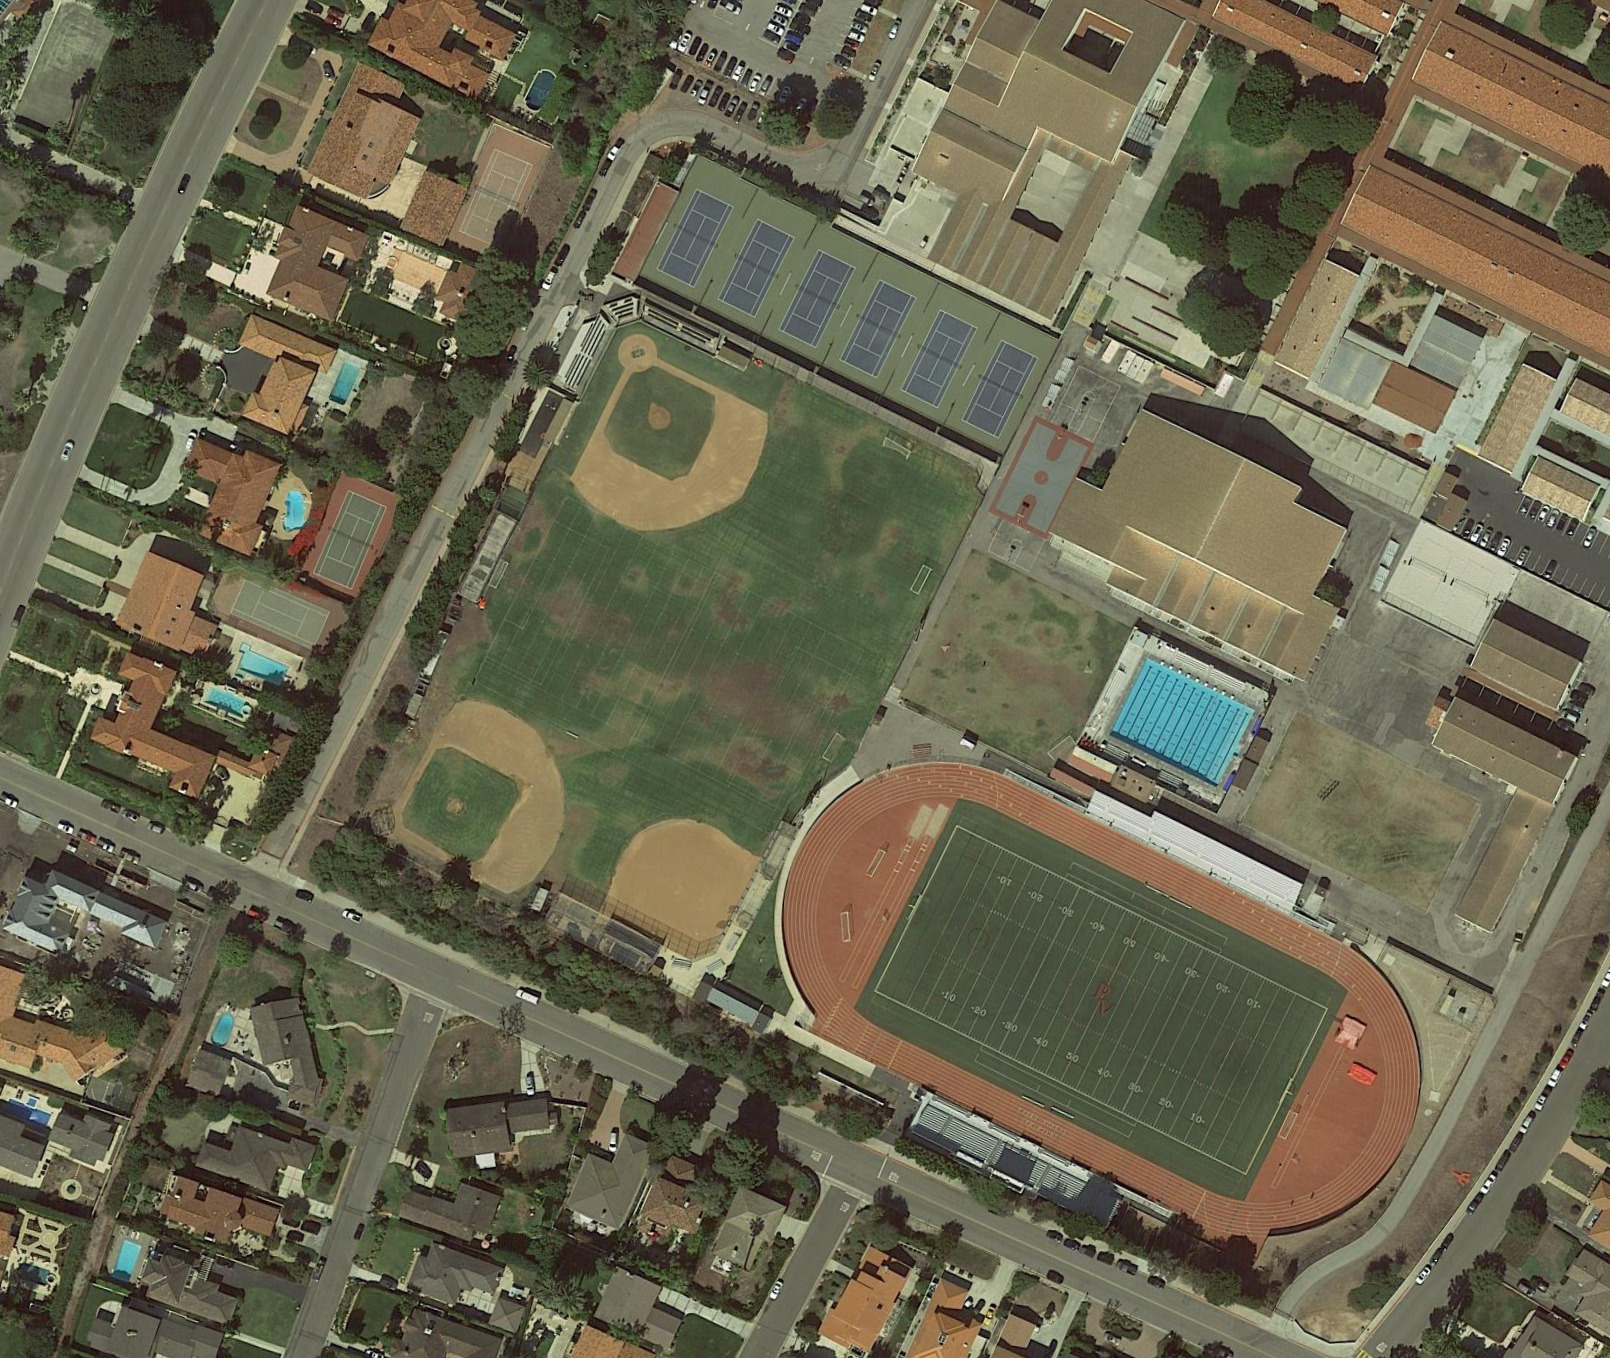
\includegraphics[width=30mm]{Figures/P0770.jpg}
                };
               
            \end{tikzpicture}
            
        \end{column}
        \pause
        
        \begin{column}{0.3\textwidth}
            

            \only<4->{
                \begin{textblock*}{50mm}(41mm,53mm)
                    \huge $\rightarrow$
                \end{textblock*}
                

                \begin{tikzpicture}[remember picture,overlay]
                    \node[xshift=\paperwidth/2 +0mm,yshift=-\paperheight/2- 5.5mm] at (current page.north west){%
                        \fbox{\parbox[][10mm][c]{0.8\textwidth}{\centering\normalsize Detection model}}
                    };
                \end{tikzpicture}
            }
            % \graphicsbox{Figures/P0131.jpg}{(0.2,0.2)}{(0.23,0.5)}{green}[20mm][0.2mm]
        \end{column}
        \pause
        \begin{column}{0.3\textwidth}
            \only<5->{
                \begin{textblock*}{50mm}(82mm,53mm)
                    \huge $\rightarrow$
                \end{textblock*}
                \centering
                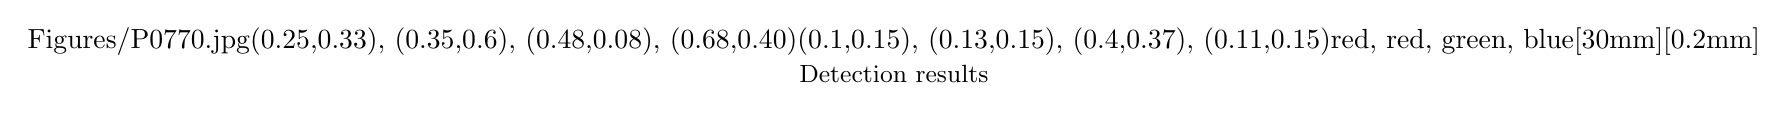
\begin{tikzpicture}
                    \node[anchor=south west,inner sep=0, label=below:{\small Detection results}] at (0,0){
                        \graphicsbox{Figures/P0770.jpg}{(0.25,0.33), (0.35,0.6), (0.48,0.08), (0.68,0.40)}{(0.1,0.15), (0.13,0.15), (0.4,0.37), (0.11,0.15)}{red, red, green, blue}[30mm][0.2mm]
                    };
                
                \end{tikzpicture}
            }
            
        \end{column}
    \end{columns}
    
    \only<3->{
    \begin{textblock}{12}(2, 12)
        $$ \mathcal{C} = \{ \text{Baseball-diamond, Swimming-pool, Ground-track-field} \}$$
      \end{textblock}
    }
        
\end{subsectionframemod}
    \begin{subsectionframemod}{Few-Shot Object Detection}
    \metroset{block=fill}
    \vspace{-10mm}
    \begin{alertblock}{$n$-way $k$-shot object detection}
        Étant donné des exemples de support $\{(x_1, a_1), \dots, (x_{nk}, a_{nk})\}$, il s'agit de détecter toutes les occurrences des classes dans $\mathcal{C}$ ($|\mathcal{C}| = n$) dans une image de requête $x_q$.
    \end{alertblock}

    \vspace{5mm}
    \pause
    \begin{columns}
        \begin{column}{0.3\textwidth}
            \centering
            \begin{tikzpicture}
                \node[anchor=south west,inner sep=0, label=below:{\small Query image}] at (0,0){
                    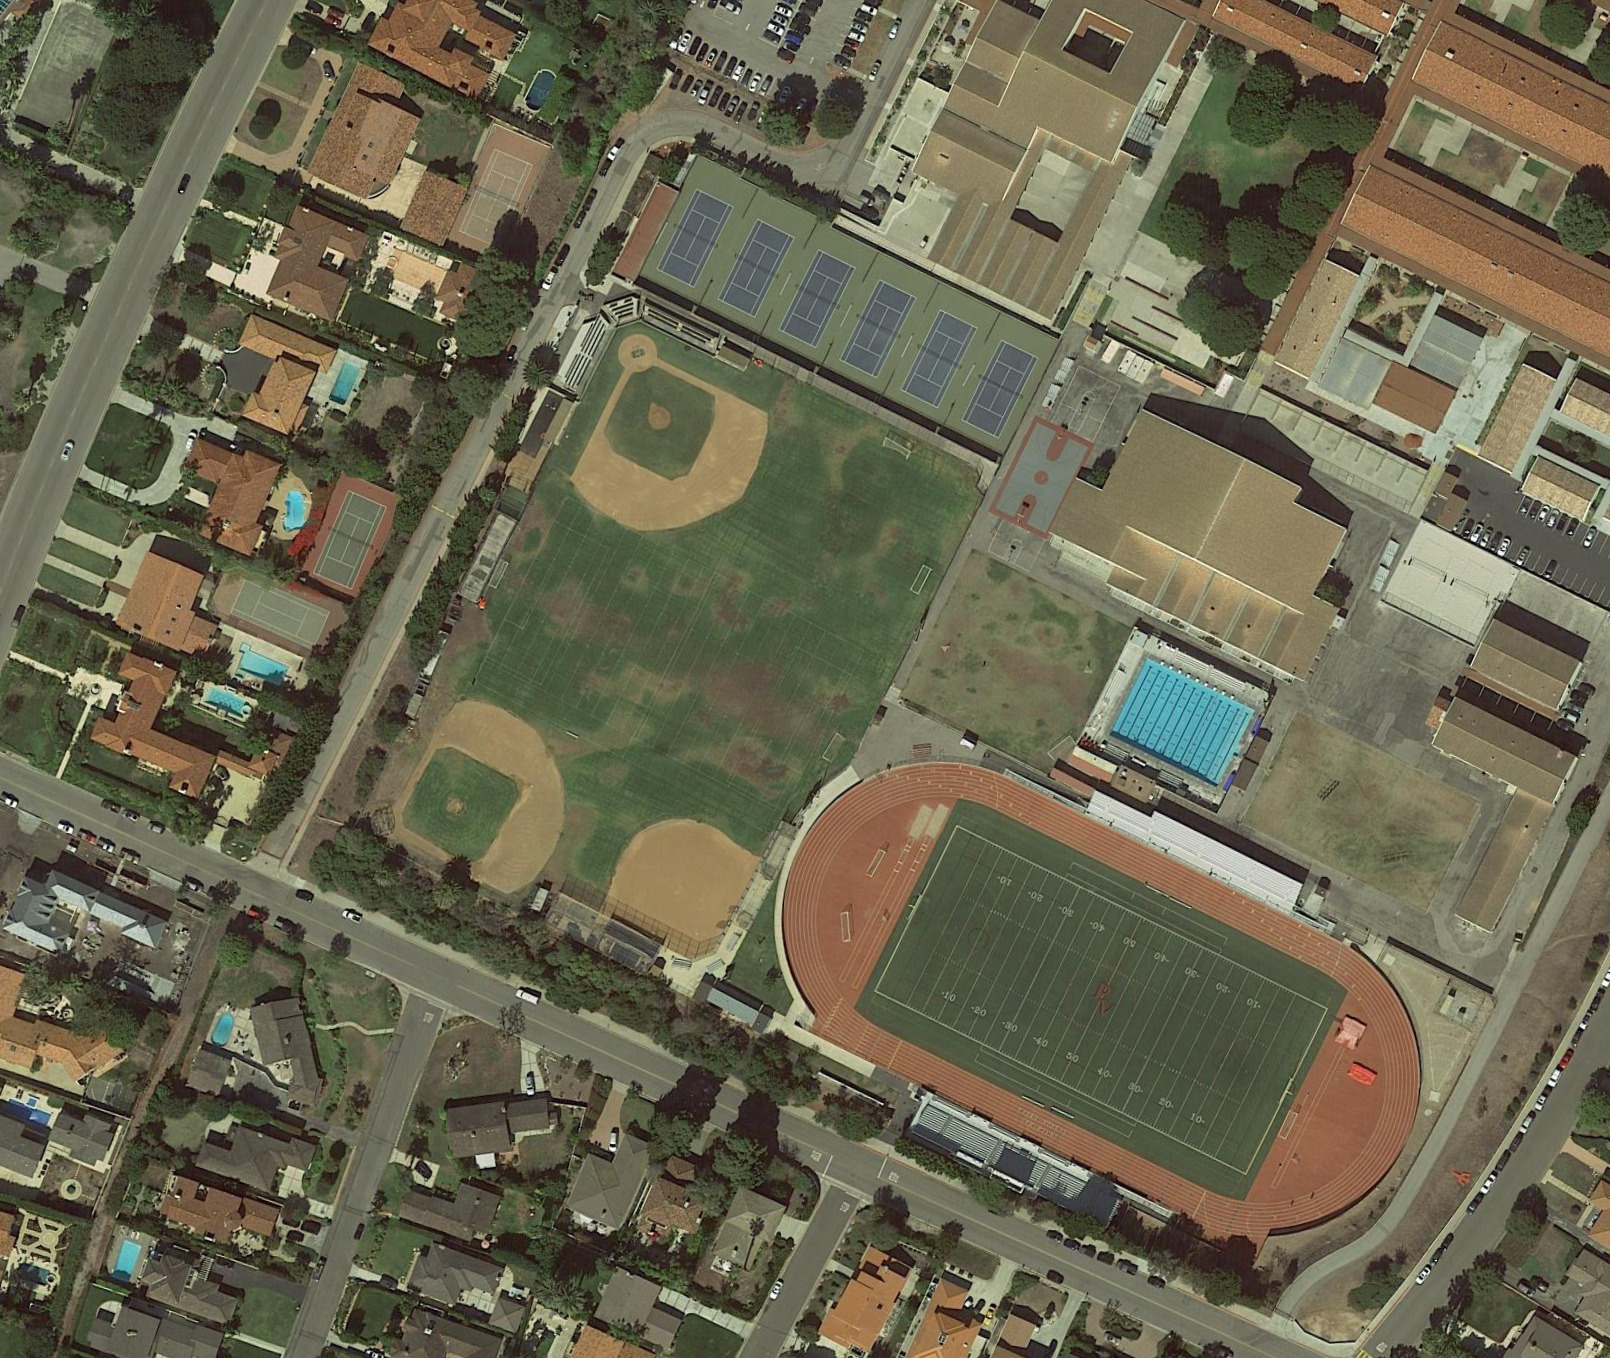
\includegraphics[width=30mm]{Figures/P0770}
                };
               
            \end{tikzpicture}
            
        \end{column}
        \pause
        
        \begin{column}{0.3\textwidth}
            
            \begin{tikzpicture}[remember picture,overlay]
                \only<3->{
                    \node[xshift=\paperwidth/2,yshift=-\paperheight/2-32mm, label=below:{\small Examples de support}](support) at (current page.north west){%

                    \graphicsbox{Figures/P0131.jpg}{(0.2,0.2)}{(0.23,0.5)}{green}[15mm][0.2mm]
                    \graphicsbox{Figures/P0168.jpg}{(0.26,0.38)}{(0.07,0.07)}{blue}[15mm][0.2mm]
                    \graphicsbox{Figures/P0352.jpg}{(0.6,0.18)}{(0.3,0.3)}{red}[15mm][0.2mm]
                    };
                }
                
                
                \only<4->{\draw[decorate, decoration ={brace,raise=1pt}] (support.north west) -- (support.north east)
                    node (supportlabel) [midway, above=10pt] {\huge $\uparrow$};}

            \end{tikzpicture}
            \only<4->{
                \begin{textblock*}{50mm}(41mm,53mm)
                    \huge $\rightarrow$
                \end{textblock*}
                

                \begin{tikzpicture}[remember picture,overlay]
                    \node[xshift=\paperwidth/2 +0mm,yshift=-\paperheight/2- 5.5mm] at (current page.north west){%
                        \fbox{\parbox[][10mm][c]{0.8\textwidth}{\centering\normalsize Modèle de détection}}
                    };
                \end{tikzpicture}
            }
            % \graphicsbox{Figures/P0131.jpg}{(0.2,0.2)}{(0.23,0.5)}{green}[20mm][0.2mm]
        \end{column}
        \pause
        \begin{column}{0.3\textwidth}
            \only<5->{
                \begin{textblock*}{50mm}(82mm,53mm)
                    \huge $\rightarrow$
                \end{textblock*}
                \centering
                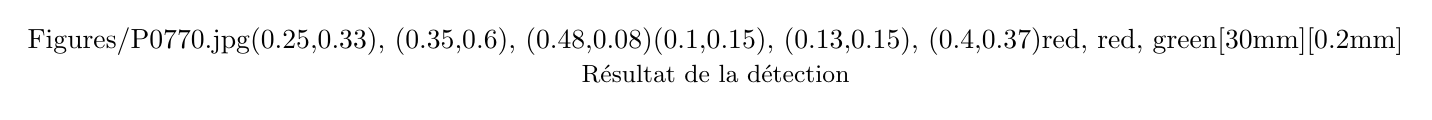
\begin{tikzpicture}
                    \node[anchor=south west,inner sep=0, label=below:{\small Résultat de la détection}] at (0,0){
                        \graphicsbox{Figures/P0770.jpg}{(0.25,0.33), (0.35,0.6), (0.48,0.08)}{(0.1,0.15), (0.13,0.15), (0.4,0.37)}{red, red, green}[30mm][0.2mm]
                    };
                
                \end{tikzpicture}
            }
            
        \end{column}
    \end{columns}
        
\end{subsectionframemod}

    \subsection{Context \& Motivation - Détection d'objet few-shot cross-domain}\label{subsec:cd-fsod}
    \begin{subsectionframemod}{Cross-Domain Few-Shot Object Detection}
        \metroset{block=fill}
    \vspace{-10mm}
    \begin{alertblock}{Cross-Domain Few-Shot Object Detection}
        In Cross-Domain Few-Shot Object Detection (CD-FSOD), two distinct datasets are used during base training and fine-tuning.
        CD-FSOD is more challenging as the model must not only adapt to new classes but also to new images.
    \end{alertblock}
    \vspace{5mm}

    \pause

    \begin{center}
        
\begin{tikzpicture}[
            squarednode/.style={rectangle, draw=black, thick, minimum size=5mm},
            node distance=20mm,
        ]
            % Nodes
            \node[squarednode, label=below:{\small Base Dataset}] (maintopic) {COCO Dataset};
            \node[squarednode, right= of maintopic] (rightsquare) {Detection Model};
%
%            % Lines
            \draw[->] (maintopic.east) -- node[above]{\small{Base Training}}(rightsquare.west);
        \end{tikzpicture}
    \end{center}

        \pause
    \begin{center}
        
\begin{tikzpicture}[
            squarednode/.style={rectangle, draw=black, thick, minimum size=5mm},
            node distance=20mm,
        ]
            % Nodes
            \node[squarednode, label=below:{\small Target Dataset}] (maintopic) {DOTA Dataset};
            \node[squarednode, right= of maintopic] (rightsquare) {Detection Model};
%
%            % Lines
            \draw[->] (maintopic.east) -- node[above]{\small{Finetuning}}(rightsquare.west);
        \end{tikzpicture}
    \end{center}

%
%    \begin{tikzpicture}
%        \node[anchor=south west,inner sep=0, label=below:{\small Base Dataset}] at (0,0){
%            \fbox{\parbox[][10mm][c]{0.8\textwidth}{\centering\normalsize COCO Dataset}}
%        };
%    \end{tikzpicture}
%
%    \begin{columns}
%        \begin{column}{0.3\textwidth}
%            \centering
%
%            \begin{tikzpicture}
%                \node[anchor=south west,inner sep=0, label=below:{\small Target Dataset}] at (0,0){
%                    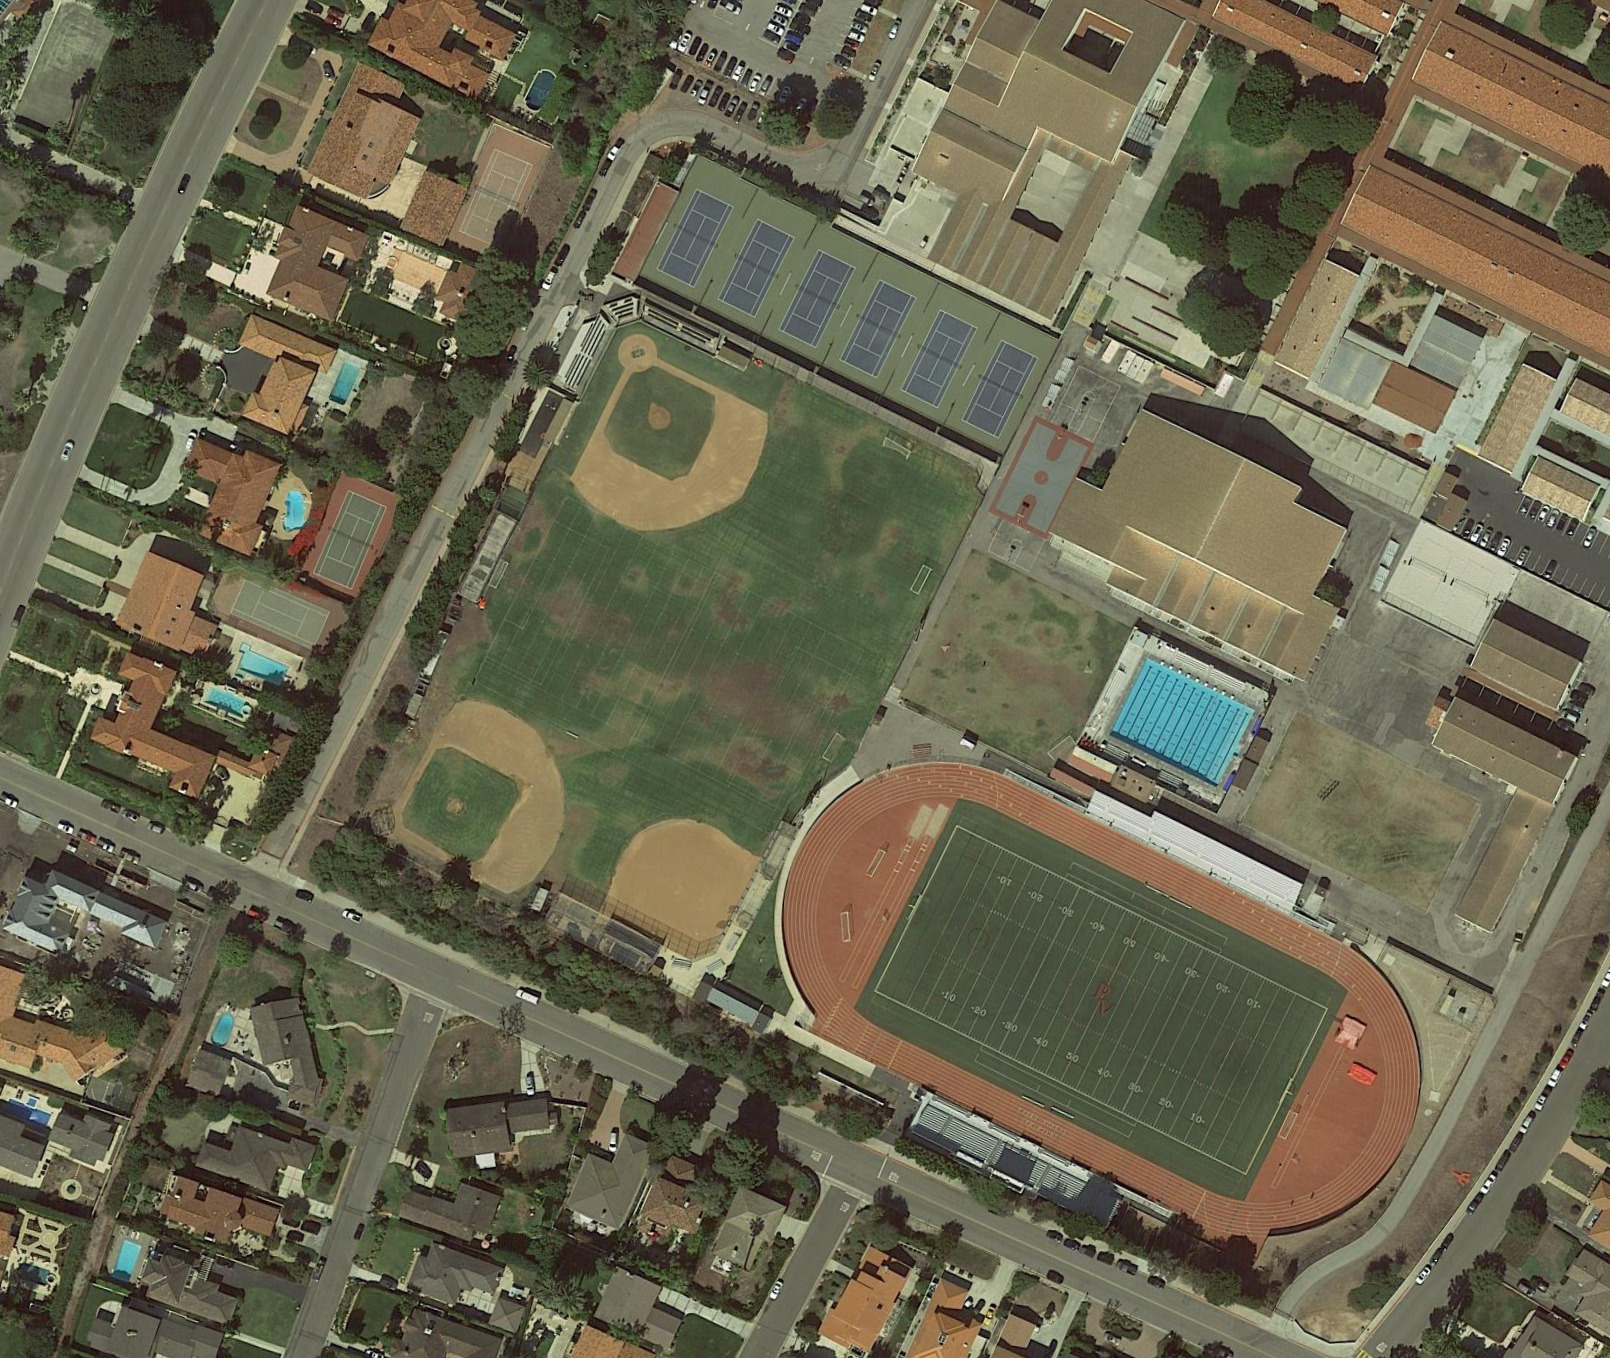
\includegraphics[width=30mm]{Figures/P0770}
%                };
%
%            \end{tikzpicture}
%
%        \end{column}
%        \pause
%
%        \begin{column}{0.3\textwidth}
%            \only<4->{
%                \begin{textblock*}{50mm}(57mm,53mm)
%                    \huge $\longrightarrow$\\
%                    \small {Base Training}
%                \end{textblock*}
%            }
%
%        \end{column}
%        \pause
%
%        \begin{column}{0.3\textwidth}
%            \only<4->{
%
%
%                \begin{tikzpicture}[remember picture,overlay]
%                    \node[anchor=south west,inner sep=0] at (0,0){%
%                        \fbox{\parbox[][10mm][c]{0.8\textwidth}{\centering\normalsize Detection model}}
%                    };
%                \end{tikzpicture}
%            }
%        \end{column}
%    \end{columns}

\end{subsectionframemod}

    \begin{subsectionframemod}{Few-Shot Object Detection}

    Plenty of methods introduced for FSOD, based on \bfalert{Fine-tuning}, \bfalert{Metric-learning} and \bfalert{Attention}. 
    \begin{itemize}
        \item[-] \textbf{Fine-tuning}: train carefully on the few available examples to avoid overfitting or catastrophic forgetting.
        \item[-] \textbf{Metric learning}: compute prototypes from support examples and classify boxes by comparison with the prototypes.
        \item[-] \textbf{Attention}: combine query and support information and separately detect objects for each class.   
    \end{itemize}
    
\end{subsectionframemod}


\begin{subsectionframemod}{Few-Shot Object Detection}
    
    \vspace{-3mm}
    \begin{table}[h]

    \label{tab:comparison}
    \begin{adjustbox}{width=0.75\textwidth}
        \rowcolors{2}{gray!25}{white}
        % \begin{tabular}{lllTLLT}
        \begin{tabular}{@{}lc}
            \begin{tabular}{@{}lc}
                \toprule[1pt]
                \textbf{Name}                               & \textbf{Backbone} \\ \hline
                Meta-RCNN~\parencite{wu2020meta}            & ResNet50          \\
                TFA w/cos~\parencite{wang2020frustratingly} & ResNet50          \\
                FSCE~\parencite{sun2021fsce}                & ResNet50          \\
                DeFRCN~\parencite{qiao2021defrcn}           & ResNet50          \\
                Distill-cdfsod~\parencite{xiong2023cd}      & ResNet50          \\ \hline
                ViTDeT-FT~\parencite{li2022exploring}       & ViT-B/14          \\ \hline
                Detic~\parencite{zhou2022detecting}         & ViT-L/14          \\
                Detic-FT~\parencite{zhou2022detecting}      & ViT-L/14          \\
                DE-ViT~\parencite{zhang2024detect}          & ViT-L/14          \\
                DE-ViT-FT~\parencite{zhang2024detect}       & ViT-L/14          \\
                CD-ViTO~\parencite{fu2024crossdomain}       & ViT-L/14          \\\bottomrule[1pt]
            \end{tabular}%
        \end{tabular}%
    \end{adjustbox}
    \caption{Comparaison des méthodes FSOD du point de vue de l'attention. Tous les
    cadres fonctionnent avec des caractéristiques multiscalaires, sauf celui avec la
    mention sans FPN.}

\end{table}
\end{subsectionframemod}

    \begin{subsectionframemod}{Difference between Natural and Aerial Images}
    La plupart des méthodes sont évaluées sur des images naturelles : les ensembles de données Pascal VOC et MS COCO.
    $\Rightarrow$ cela ne garantit pas de bonnes performances sur les images aériennes.
    \vspace{2mm}


    Les tailles des objets sont extrêmement différentes entre les images aériennes et naturelles.

    \begin{figure}
        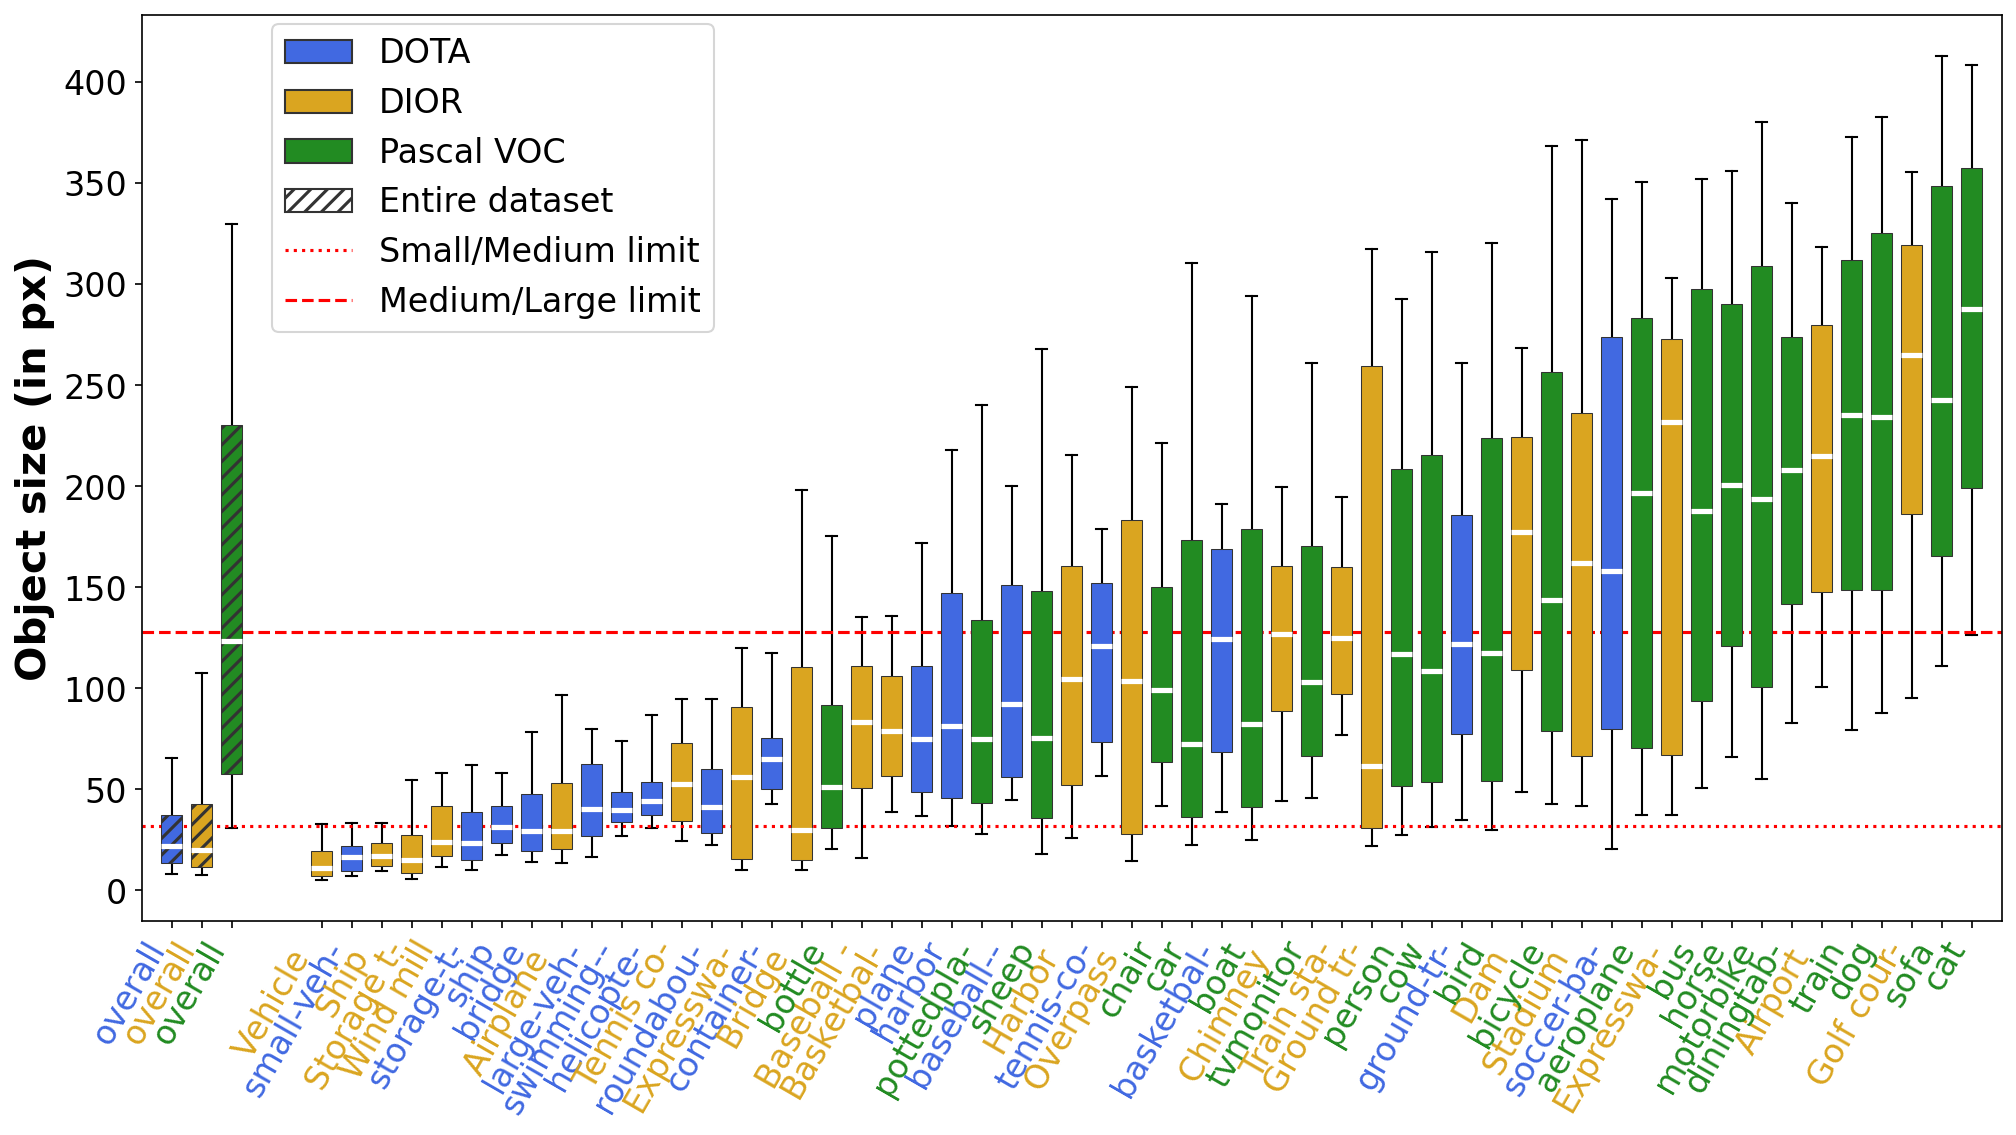
\includegraphics[width=0.8\textwidth]{Figures/object_sizes.png}
    \caption{Diagramme en boîte des tailles d'objets dans DOTA (\cite{xia2018dota}), DIOR (\cite{li2020object}) et Pascal VOC (\cite{everingham2010pascal}); par classe \textbf{(à droite)} et globalement \textbf{(à gauche)}.}
    \end{figure}

    

    
\end{subsectionframemod}
    \begin{subsectionframemod}{Performance Analysis}
    
    
    Il est impossible de comparer les performances sur différents ensembles de données.
    Cependant, il est possible de \alert{comparer les performances FSOD par rapport à une référence non few-shot}
    et de comparer cela sur plusieurs ensembles de données.

    \begin{figure}
        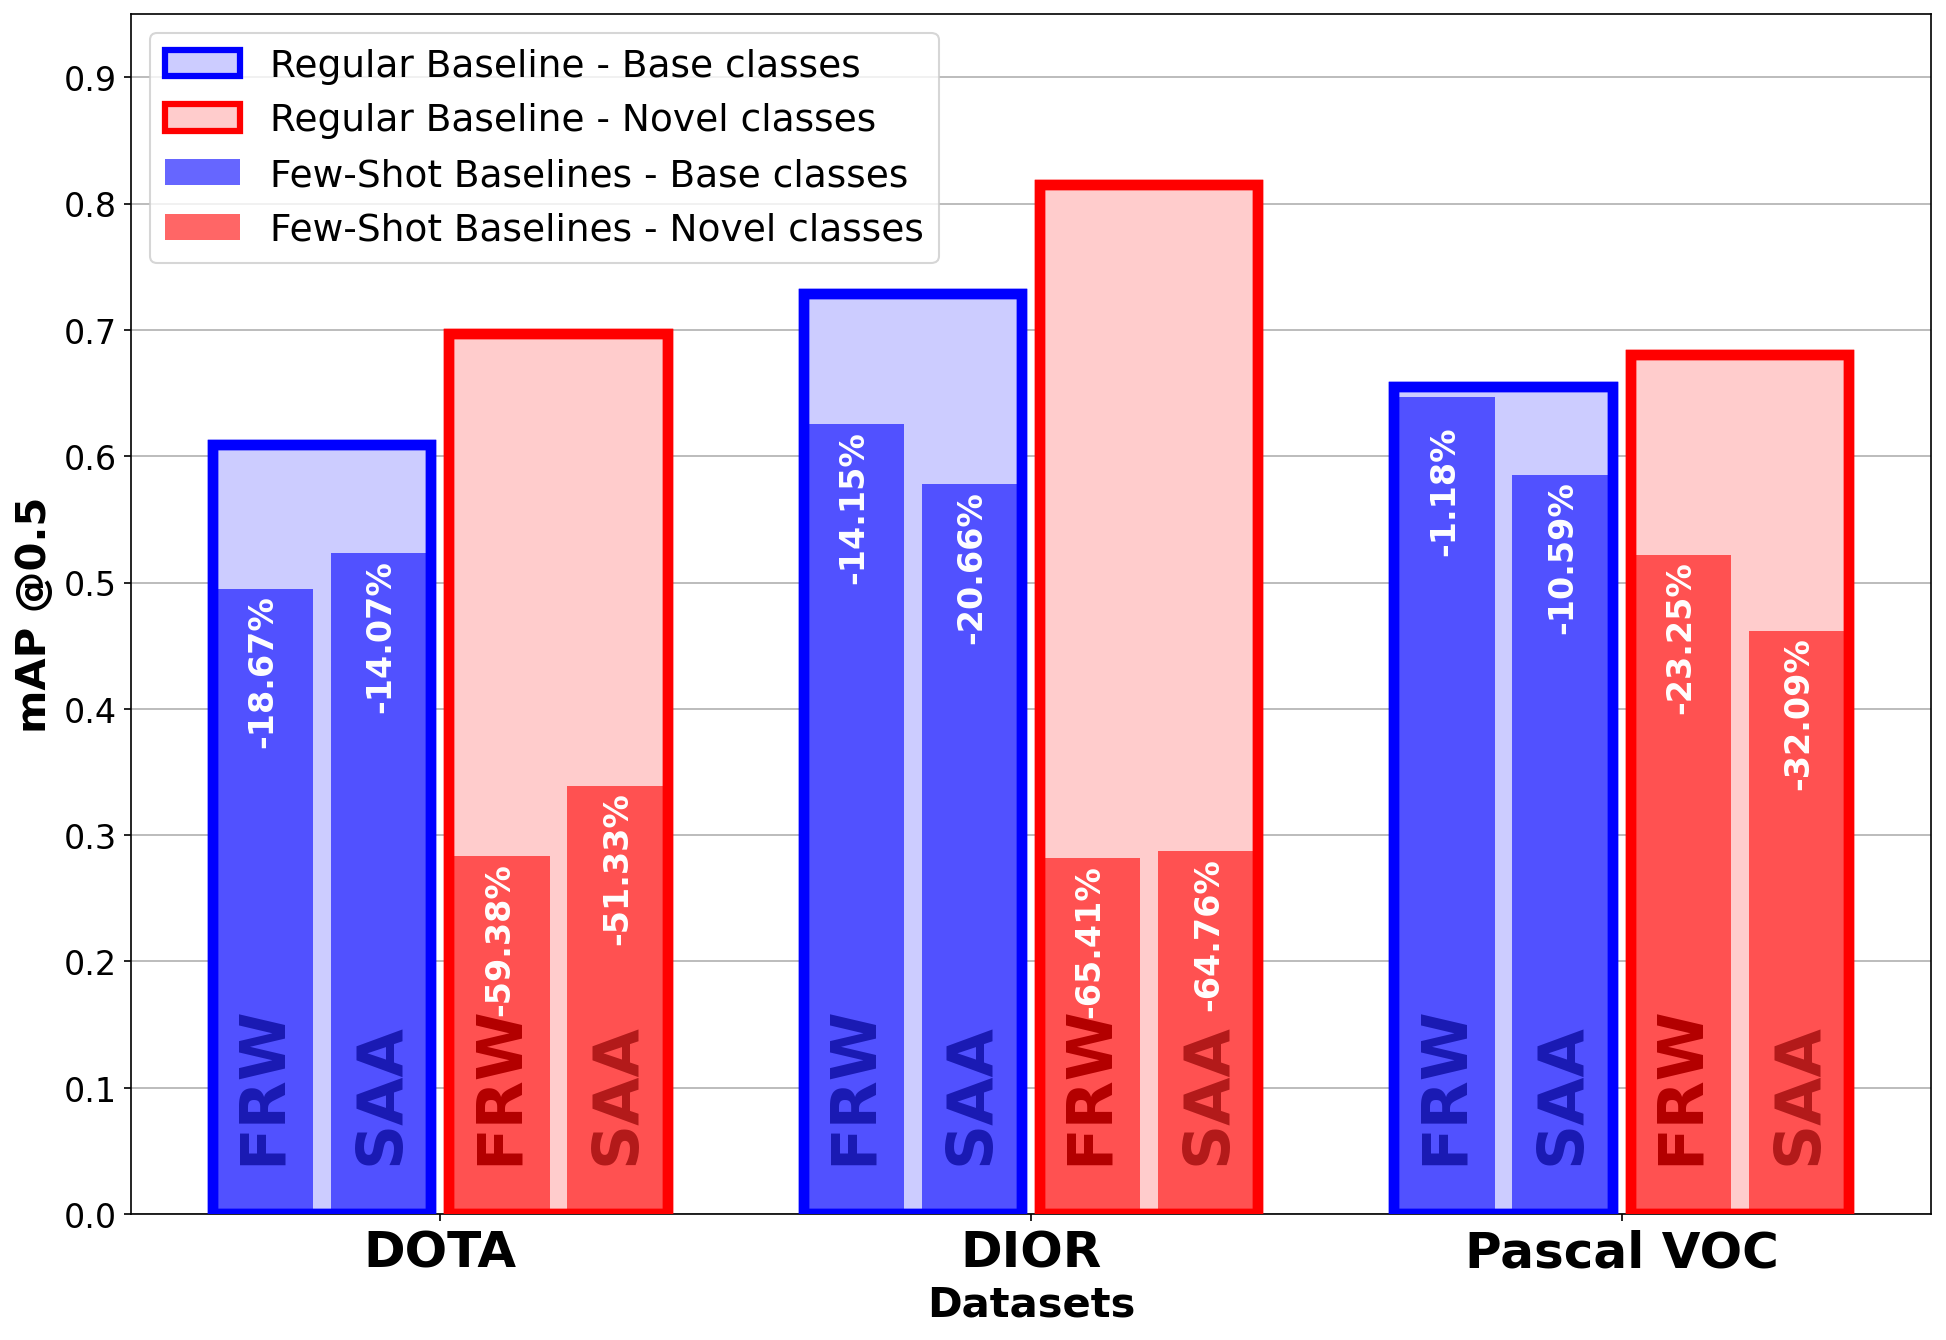
\includegraphics[width=0.8\textwidth]{Figures/dataset_comparison.png}
        \caption{Performances FSOD comparées sur DOTA, DIOR et Pascal VOC. (\cite{lejeune2022improving})}
    \end{figure}

\end{subsectionframemod}

\begin{subsectionframemod}{Performance Analysis}
    Les grandes différences de taille moyenne entre les classes suggèrent d'analyser les performances par classe.
    \alert{Corrélation claire entre la taille moyenne des classes et les performances} par rapport à la référence.
    \begin{figure}
        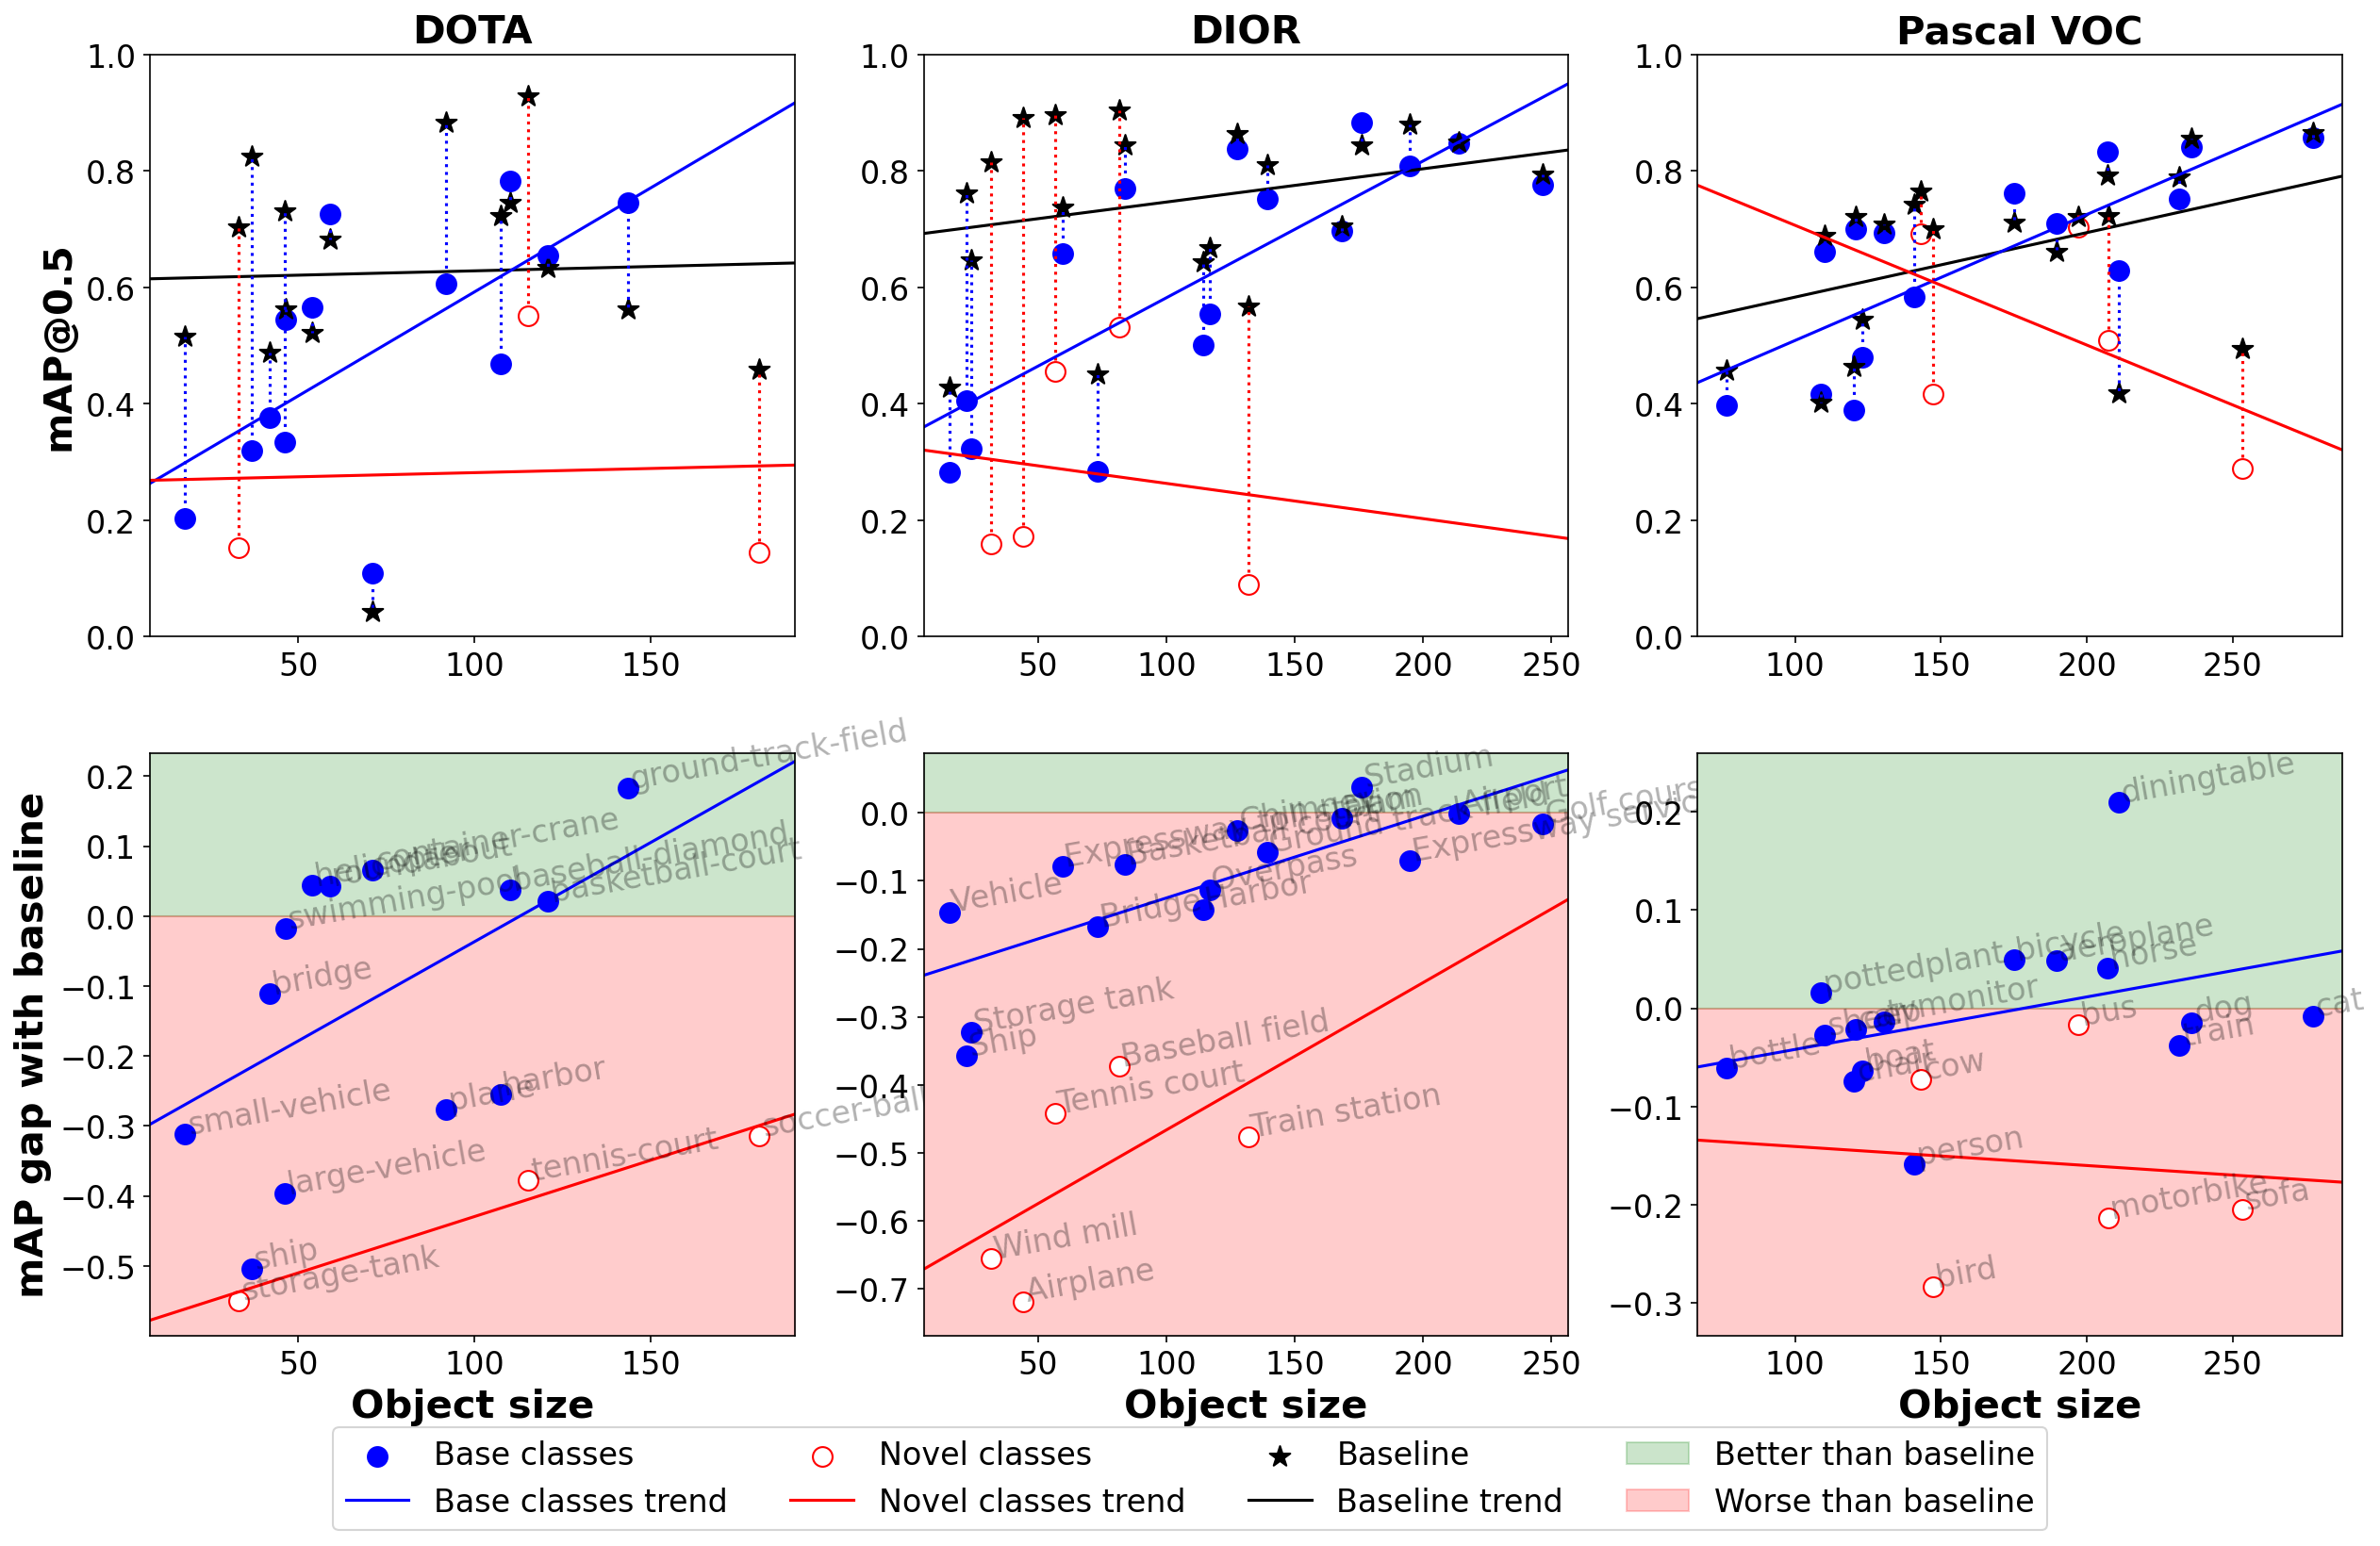
\includegraphics[width=0.85\textwidth]{Figures/performance_comparison.png}
    \caption{Analyse des performances par classe et comparaison avec la référence non few-shot sur DOTA, DIOR et Pascal VOC. (\cite{lejeune2022improving})}
    \end{figure}

\end{subsectionframemod}

    \section{Proposed Approaches}

%     \subsection{Prototypical Faster R-CNN}
%     \usepackage{tikz}\begin{subsectionframemod}{Proposed Approaches}
    \begin{overlayarea}{\textwidth}{\textheight}
        \vspace{2mm}
        \bfalert{Main principle:} integrate prototypical networks inside Faster R-CNN.
        \vspace{2mm}
        \begin{overlayarea}{\textwidth}{0.3\textheight}
            \begin{columns}[T]
            
                \begin{column}{0.5\textwidth}
                    \only<2->{
                    \alert{RPN:} multi-class prototypes but only outputs objectness score (i.e. binary classification).
    
                    \centering
                    \begin{minipage}{0.99\textwidth}
                        \centering
                        \begin{equation*}
                            o_{j} = \max\limits_{c \in C_i} \exp\Big(\frac{-d(z_{j}, p_c)^2}{2\sigma^2}\Big)
                        \end{equation*}
                    \end{minipage}
                    }
                \end{column}
                
                \begin{column}{0.5\textwidth}
                    \only<3>{
                    \alert{Classification head:} prototypical networks attribute class scores to RoI extracted from RPN boxes \parencite{karlinsky2019repmet}.
    
                    \centering
                    \begin{minipage}{0.99\textwidth}
                        \begin{equation*}
                            p(c |x_{j,a}) =\frac{\exp\Big(\frac{-d(z_{j}, p_c)^2}{2\sigma^2}\Big)}{\sum\limits_{c' \in C_i \cup \{\varnothing\}} \exp\Big(\frac{-d(z_{j}, p_{c'})^2}{2\sigma^2}\Big)}
                        \end{equation*}
                    \end{minipage}
                    }
                \end{column}
            
            
            
            \end{columns}
        \end{overlayarea}

        \vspace{0mm}
        
        \begin{figure}
            \centering
            \begin{tikzpicture}
                \only<2->{
                    \node[anchor=south west, inner sep=0] (image) at (0,0) {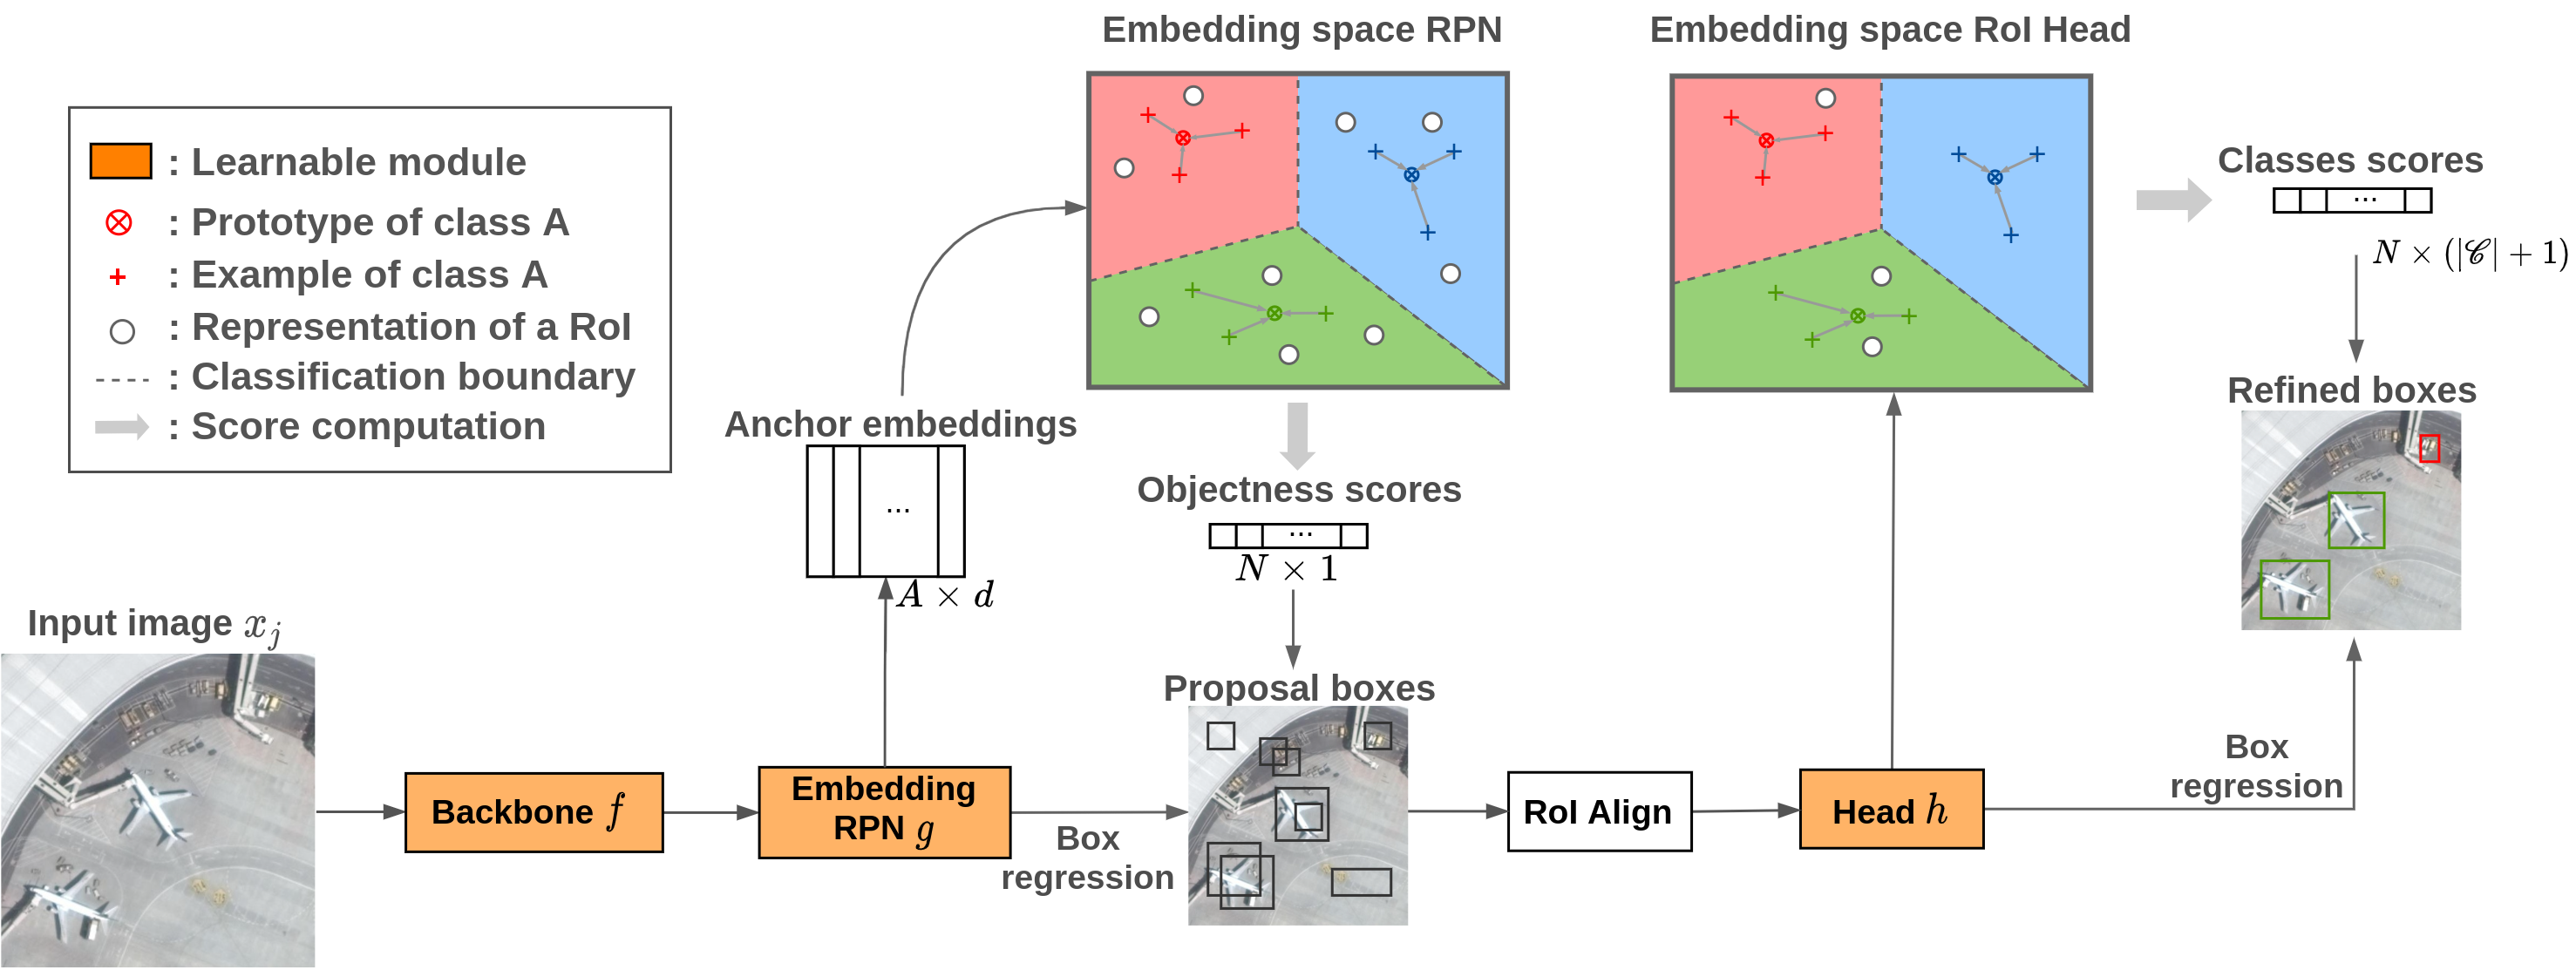
\includegraphics[width=0.95\textwidth]{Figures/prototypical_frcnn_rework.png}};
                }
                \only<2>{
                    \begin{scope}[x={(image.south east)},y={(image.north west)}]
                        \draw[color=black!2, fill=black!2, overlay] (0.62,0.05) rectangle (1,1);
                        \draw[color=black!2, fill=black!2, overlay] (0.55,0.05) rectangle (1,0.25);
                    \end{scope}
                }
                
            \end{tikzpicture}
            \only<2->{
                \vspace{-2mm}
                \caption{Prototypical Faster-RCNN architecture.}
            }
            
        \end{figure}
    
        
    \end{overlayarea}
\end{subsectionframemod}

%    \subsection{Proposed Approaches - Diffusion Based Models}
%    \begin{subsectionframemod}{Proposed Approaches}

    The main idea of DiffusionDet is to apply the diffusion principle to box generation.

    Random boxes are first sampled, and a model is trained to refine iteratively the size and position of the boxes so that they localize the objects in the input image.

    Specifically, the boxes are iteratively \alert{denoised} by the model.



    \begin{figure}
        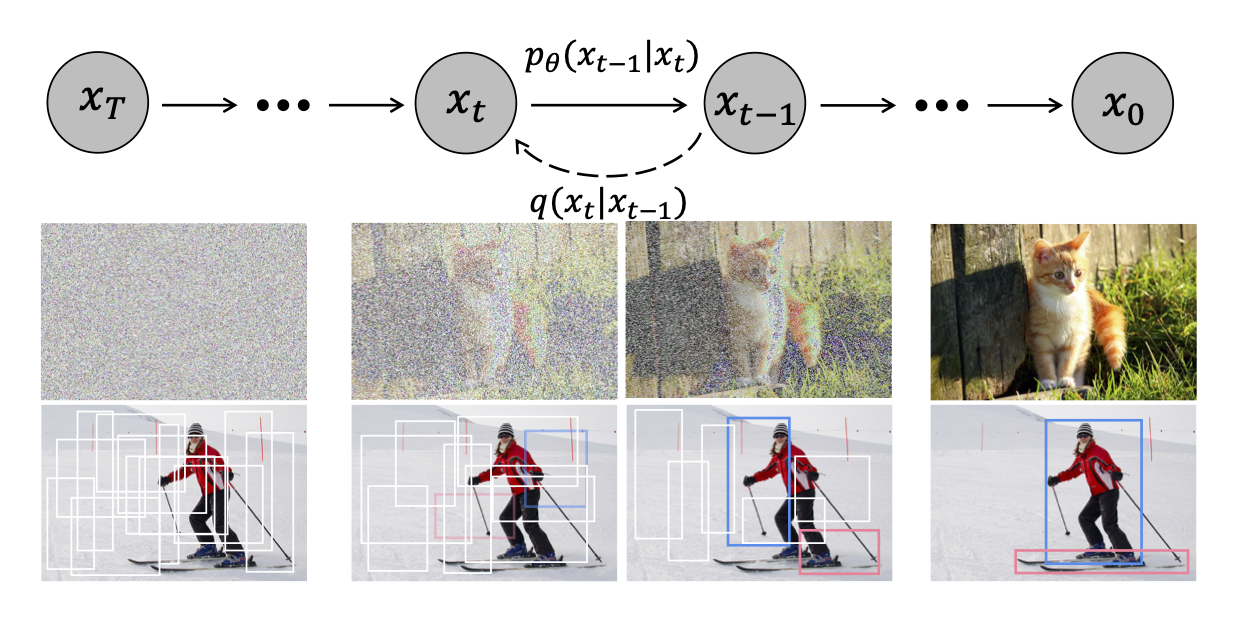
\includegraphics[width=0.70\textwidth]{Figures/teaser_diffusion}
        \caption{
        Diffusion model for object detection.
            In the first line a diffusion model where $q$ is the diffusion process and $p_{\theta}$ is the reverse process.
            Then a diffusion model for image generation task.
            And in the last one we propose to formulate object detection as a denoising diffusion process from noisy boxes to object boxes.\\
            \small{\textit{taken from DiffusionDet paper \cite{chen2022diffusiondet}}}
        }\label{fig:diffusion}
    \end{figure}

\end{subsectionframemod}

\begin{subsectionframemod}{Proposed Approaches}

    The denoising part of DiffusionDet is a lightweight hybrid network, it consists of a self-attention layer (transformer-like) followed by a dynamic layer (called an Instance Interaction layer).
    The detection head processes object features independently, but the Instance Interaction layer enables interactions between instances.
    The detection head is applied iteratively to refine the bounding boxes

    \begin{figure}
        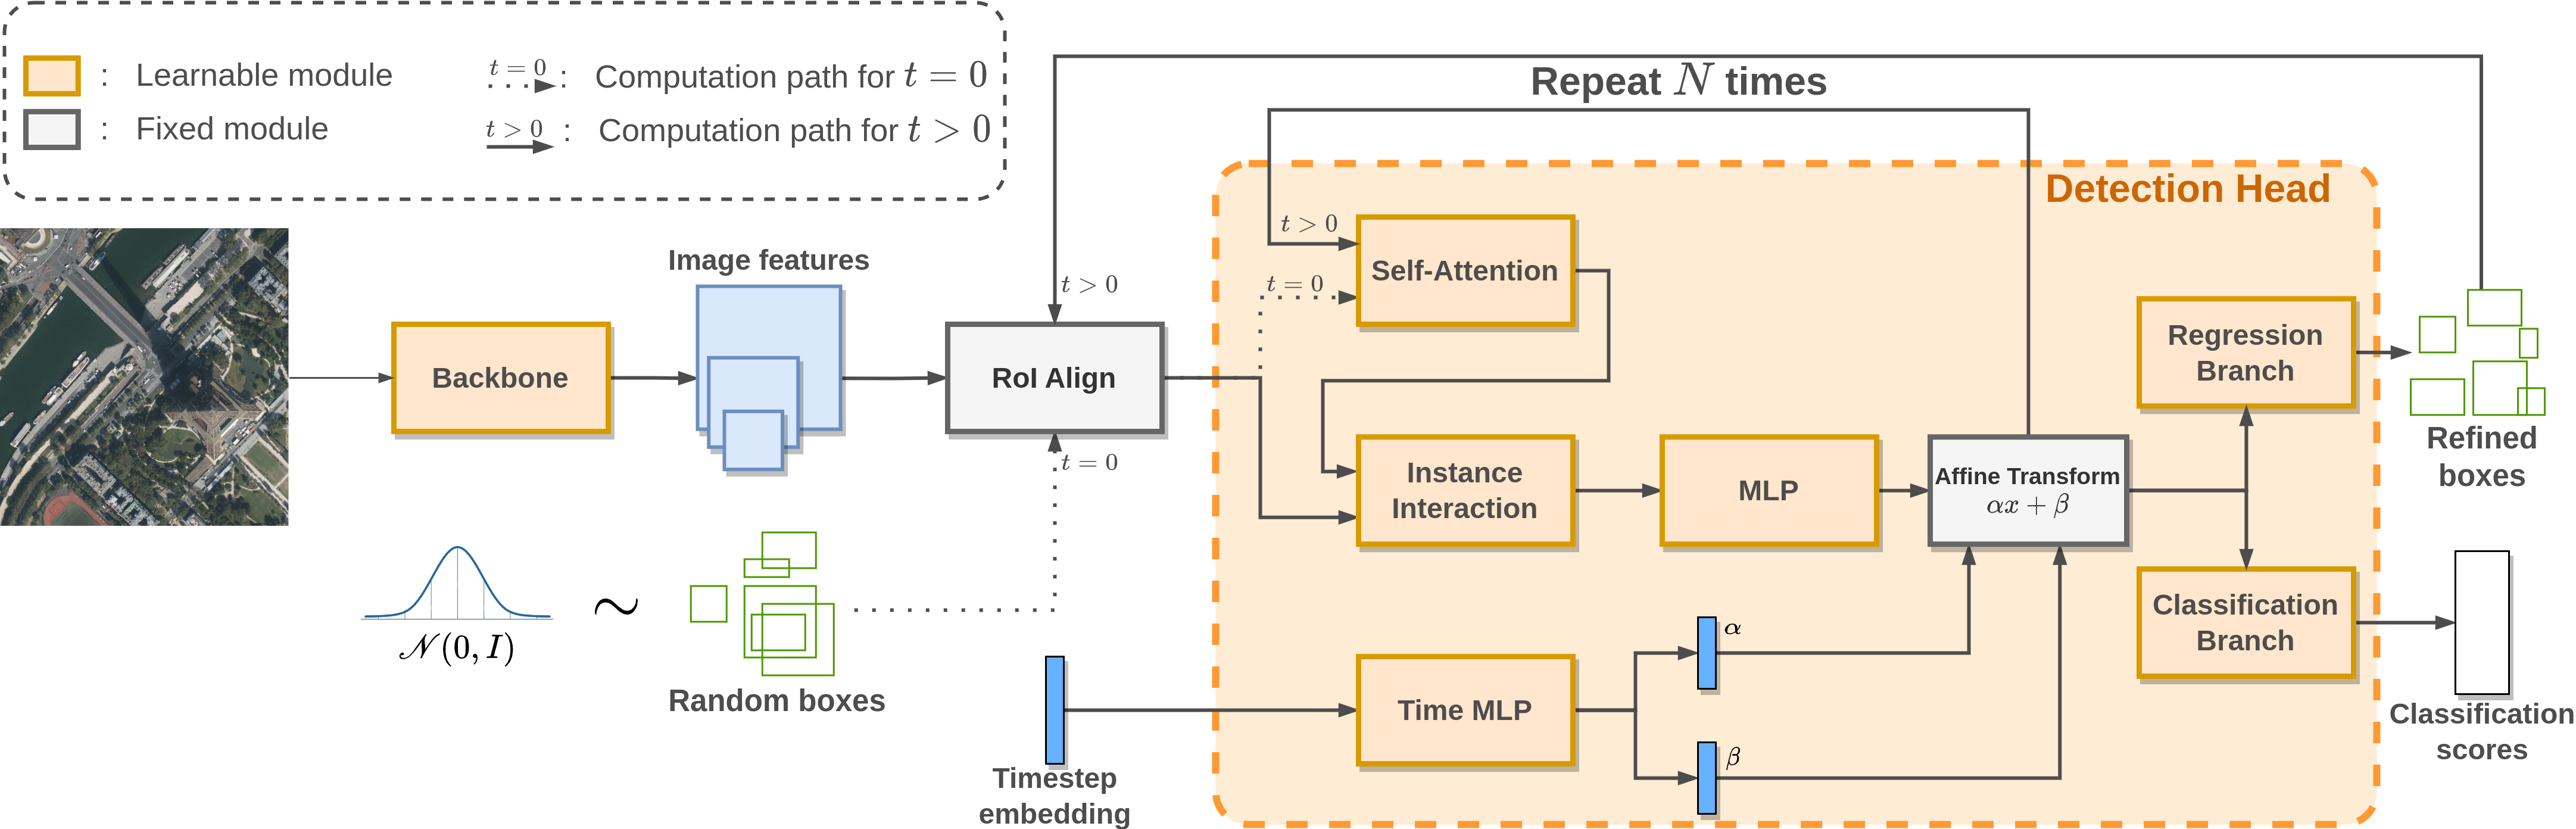
\includegraphics[width=0.95\textwidth]{Figures/DiffusionDet}
        \caption{DiffusionDet architecture and detailed detection head design.}\label{fig:diffusiondet}
    \end{figure}

\end{subsectionframemod}
%
%    \subsection{Proposed Approaches - Few-Shot DiffusionDet}
%    \begin{subsectionframemod}{Proposed Approaches}
     Let us introduce some notations.

     We denote by $\mathcal{F}_c$ and $\mathcal{F}_r$ the sub-models responsible for classification and regression respectively:

    \begin{align}
        \mathcal{F}_c &= f_c \circ f, \\
        \mathcal{F}_r &= f_r \circ f, \\
        \text{with } f &= f^{L-1} \circ f^{L-2} \circ \dots \circ f^1.
    \end{align}

     \pause

     To leverage DiffusionDet in the few-shot regime, we propose to adopt a Transfer Learning approach.
     Once, the model is base-trained, it is prepared for fine-tuning.

     A large part of the model is frozen.
     The crucial part is that we can finely control the amount of frozen layers with a hyperparameter $\gamma$.

    Denoting frozen layers with a bar (\eg $\overline{f^1}$), the frozen detection model is expressed as

    \begin{equation}
        f = f^L \circ \dots \circ f^{\gamma+1} \circ \overline{f^\gamma} \circ \dots \circ \overline{f^1}.
        \label{eq:frezze}
    \end{equation}


\end{subsectionframemod}
%
%    \section{Results and Analysis}
%    \subsection{Results and Analysis - Few-Shot Senarios}
%    \begin{subsectionframemod}{Proposed Approaches}

    \begin{figure}
        \includegraphics[width=0.95\textwidth]{Figures/perf_vs_shots_diff}
        \caption{Performance (mAP$_{0.5}$) of
        FSDD (ours), XQSA \cite{lejeune2023xqsa}, FRW \cite{kang2019few}, DANA \cite{chen2021should} and WSAAN \cite{xiao2020fsod} on DOTA, DIOR, Pascal VOC and MS
        COCO against the number of shots. Black dashed lines represent performance achieved with full supervision.}\label{fig:diff_perf_vs_shot}
    \end{figure}
     
\end{subsectionframemod}

%
%    \begin{subsectionframemod}{Proposed Approaches}
     Determining how much of the model should be fine-tuned is a complex task in FSOD.
     Here, we investigate this choice with thorough experiments on four datasets.

     \begin{table}[]
    \centering
    \resizebox{\columnwidth}{!}{%
    \begin{tabular}{@{\hskip 2mm}lccccc@{\hskip 2mm}}
    \toprule[1pt]
    \textbf{Freezing point}& \textbf{Plasticity}   & \textbf{DOTA} & \textbf{DIOR} & \textbf{Pascal VOC} & \textbf{COCO} \\ \midrule
    FT whole               & 100.00 \%             & 60.09         &  52.17             & 43.10           &  17.15             \\
    Bias only              & 35.98 \%              & \textbf{60.45}&  55.12             & 49.90           &  20.19             \\
    BatchNorm only         & 35.97 \%              & 59.35         &  55.63             & 51.96           &  19.70             \\
    Up to stage 1          & 99.98 \%              & 58.85         &  53.37             & 43.81           &  17.72             \\
    Up to stage 4          & 99.47 \%              & 57.41         &  53.21             & 41.23           &  17.73             \\
    Up to stage 3          & 96.57 \%              & 59.88         &  54.36             & 47.57           &  19.49             \\
    Up to stage 4          & 79.66 \%              & 56.13         &  \textbf{57.51}    & \textbf{53.72}  &  \textbf{21.88}    \\
    FT head only           & 35.97 \%              & 51.82         &  55.70             & 51.72           &  19.96             \\
    FT last layer only     & 0.03 \%               & 0.05          &  0.11              & 0.53            &   0.01             \\ \bottomrule[1pt]
    \end{tabular}%
    }
    \vspace{-0.5em} \caption{Influence of the freezing point on the
    FS performance on DOTA, DIOR, Pascal VOC, and COCO. mAP is reported with a 0.5 IoU threshold and $k=10$ shots.}
    \label{tab:diff_freezing_sweetspot}
    \vspace{-1.5em}
    \end{table}
\end{subsectionframemod}

%
%    \subsection{Results and Analysis - Cross-Domain Senarios}
%    \begin{subsectionframemod}{Proposed Approaches}

    The great results of FSDD on aerial images suggest trying the more complex scenario of CD-FSOD almost untouched in the literature.

    -$1^{st}$ Senario: COCO $\to$ X,

    \begin{table}[]
        \centering
        \resizebox{0.9\columnwidth}{!}{%
        \begin{tabular}{@{\hspace{2mm}}ccccccc@{\hspace{2mm}}}
        \toprule[1pt]
        \multicolumn{1}{l}{\textbf{$k$ Shots}} & \textbf{DIOR} & \textbf{DOTA} & \textbf{DeepFruits} & \textbf{SIXRay} & \textbf{VisDrone}\\ \midrule
        \textbf{1}                           & 11.10     & 4.03        & 38.47            &  4.80 & 2.83       \\
        \textbf{5}                           & 30.42     & 14.45       & 55.58             & 13.25 & 5.74       \\
        \textbf{10}                          & 38.73     & 25.02       & 68.37             & 21.26 & 7.50       \\
        \textbf{20}                          & 48.23     & 33.31       & 73.95             & 30.06 & 9.14       \\
        \textbf{50}                          & 56.97     & 43.23       & 76.65             & 41.93 & 11.47       \\ \bottomrule[1pt]
        \end{tabular}%
        } \caption{Cross-domain performance results
        on 5 scenarios COCO $\to$ DIOR / DOTA / DeepFruits (\cite{lee2022rethinking}) / SIXRay (\cite{miao2019sixray}) / VisDrone (\cite{pengfei2021visdrone}).}
        \label{tab:cd_fsod_results}
        \vspace{-1.1em}
        \end{table}


\end{subsectionframemod}

\begin{subsectionframemod}{Proposed Approaches}

    -$2^{nd}$ Senario: DOTA $\to$ DIOR and DIOR $\to$ DOTA,

    \begin{table}[]
        \centering
        \resizebox{0.9\columnwidth}{!}{%
        \begin{tabular}{@{\hspace{2mm}}cccccccccc@{\hspace{2mm}}}
        % \toprule
        \multicolumn{1}{l}{} & \multicolumn{2}{c}{{\ul \textbf{DOTA $\to$ DIOR}}} & & \multicolumn{2}{c}{{\ul \textbf{DIOR $\to$ DOTA}}}  \\ \midrule
        \textbf{$k$ shots}   & \textbf{FT head only}         & \textbf{FT whole}&    & \textbf{FT head only}        & \textbf{FT whole}         \\ \midrule
        \textbf{1}           & \textbf{20.18}       & 9.40        &    & \textbf{5.41 }      & 5.09                 \\
        \textbf{5}           & \textbf{34.43}       & 29.57       &    & \textbf{25.88}      & 24.90                \\
        \textbf{10}          & \textbf{41.48}       & 38.44       &    & 31.99               & \textbf{33.30}       \\
        \textbf{20}          & \textbf{49.00}       & 45.36       &    & 38.77               & \textbf{41.30}       \\
        \textbf{50}          & \textbf{54.07}       & 53.51       &    & 44.07               & \textbf{49.22}       \\ \bottomrule[1pt]
        \end{tabular}%
        } \caption{FSDiffusionDet Cross-Domain (CD-FSOD)
        results on the scenarios DOTA $\to$ DIOR and DIOR $\to$ DOTA.
        Performance is reported with mAP$_{0.5}$ values.}
        \label{tab:cd_fsod_dota2dior}
        \vspace{-1.5em}
        \end{table}
\end{subsectionframemod}
%
%    \subsection{Perspectives}
%
%
%    \section{Integration in CAMELEON}
    \section{Conclusion and Perspectives}
    \begin{subsectionframemod}{Conclusion}
Persepctives d'avenir et futurs travaux:
\begin{itemize}
    \item[-]  Framework pour expérimenter rapidement en cross domain (objectif courant octobre)
    \item[-]  Papier benchmark (objectif novembre)
    \item[-]  Chercher des PEFT qui fonctionne pour la regression (objectif début 2025)
    \item[-]  Compléter le papier du benchmark pour l'inclure dans un journal (objectif début 2025)
    \item[-]  Travaux sur les vlm (vision/language models) (objectif courant 2025)
\end{itemize}


\end{subsectionframemod}

    \usebeamertemplate{endpage}

    \begin{frame}[allowframebreaks=]{References}
        \printbibliography
    \end{frame}
\end{document}
